\documentclass[12pt]{article}
\usepackage{parskip}
\usepackage{amsmath}
\usepackage{pdfpages}
\usepackage{listings}
\usepackage{color}
\usepackage[margin=.6in]{geometry}

\definecolor{dkgreen}{rgb}{0,0.6,0}
\definecolor{gray}{rgb}{0.5,0.5,0.5}
\definecolor{mauve}{rgb}{0.58,0,0.82}

\lstset{frame=tb,
  language=C++,
  aboveskip=3mm,
  belowskip=3mm,
  showstringspaces=false,
  columns=flexible,
  basicstyle={\small\ttfamily},
  numbers=none,
  numberstyle=\tiny\color{gray},
  keywordstyle=\color{blue},
  commentstyle=\color{dkgreen},
  stringstyle=\color{mauve},
  breaklines=true,
  breakatwhitespace=true,
  tabsize=3
}

\begin{document}
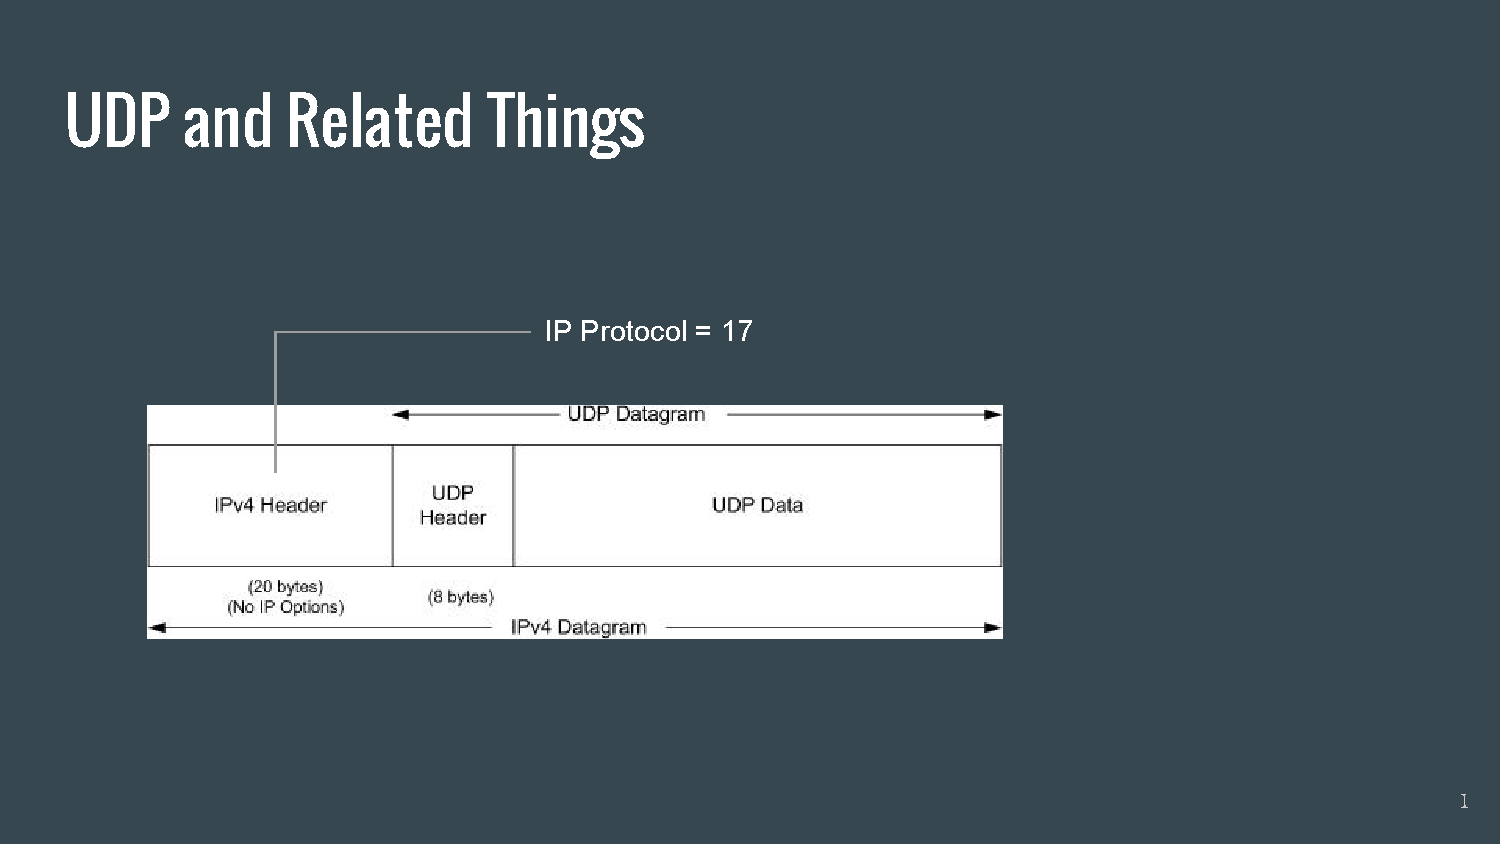
\includepdf[pages=1-3]{slides.pdf}
The header here is much simpler than it was for ip. The destination ip and destination port are the only bits of data required to get the packet to its destination. You can say that you have a source port of 0, but the destination might no allow it. The length field is the length of the header. Its completely redundant because the ip layer already has the length in it. 

\includepdf[pages=4]{slides.pdf}
The checksum calculation is a bit wonky because the udp data might be odd lengthed. It is caclulated from the udp header, data, and a pseudo header. If this happens you add a byte for padding to fix this. Its a bit weird because the checksum is included in the calculation of the checksum.

\includepdf[pages=5]{slides.pdf}
We include a pseudo header that has duplicate information for the destination and source ip address in case there are bugs in the ip layer. When we are calculating the checksum we can use 0s in the checksum calculation. Some protocols don't even bother calculating the checksum because it already has it from the ip layer or it is weak. If the checksum works out to being 0 you can run into problems because it is used to denote that the checksum is unimportant. The udp checksum is not recalculated with each hop because it is a transport protocol. Problems can occur during network address translations.

If you fragment the udp datagram the header become separated from the data, but that is ok because they will be reassembled at the destination then the conversion to the udp layer happens. 

\includepdf[pages=6]{slides.pdf}
In udp lite we get rid of the length and use checksum coverage instead to say how much of you udp packet is covered in the calculation of the checksum.  This transport layer is completely different than udp, it just shares a name. This was done for performance reasons. 

\includepdf[pages=7]{slides.pdf}
Udp is super simple and powerful. Traceroute uses it. It also has something called the echo service (tcp does as well, infact most of port numbers are shared between the two). This is a standard that says if you send a packet there it will return that exact packet back. We can use this to find the largest datagram you network can support (called maxmium transmission unit). We send a packet that is of a size we want to test minus 28 bytes for the header. We send this packet to the echo port with a no fragmentation flag. If we get a packet returned we know that this size is supported throughout the network. It is important to note that if you don't get a response that doesn't necissarily mean that the packet size is not supported (there a bunch of reasons there wasn't a response).  

\includepdf[pages=8]{slides.pdf}
\includepdf[pages=9]{slides.pdf}
There is another command called ioctl that is super shitty. Getsockname is a layer above it and works a bit better. 

\includepdf[pages=10]{slides.pdf}
Most fragments are of type udp. A theory for this is that this is the result of encapsulation. As we encapsulate more layers the datagram gets bigger and thus is more likely to require fragmentation. Another theory is that people who write udp tend to be more careless.

\includepdf[pages=11]{slides.pdf}
\includepdf[pages=12]{slides.pdf}









\end{document}